
\beginsupp
\setcounter{section}{0}
\renewcommand\thesection{\Alph{section}}
\noindent
{\Large {\textbf{Supplementary materials}}}
\\

These materials include the details of network architecture (\S\ref{suppsec:arch}), implementation (\S\ref{suppsec:implementation}), FC100 dataset splits (\S\ref{suppsec:fc100splits}), standard variance analysis (\S\ref{suppsec:ci95}), additional ablation results (\S\ref{suppsec:addexp}), and some interpretation of our meta-learned model (\S\ref{sec_visual}).
In addition, our open-source code is on GitHub\footnote{\href{https://github.com/y2l/meta-transfer-learning-tensorflow}{https://github.com/y2l/meta-transfer-learning-tensorflow}}.

%%%


\section{Network architectures}
\label{suppsec:arch}
In Figure~\ref{figure_netarch_4CONV}, we present the 4CONV architecture for feature extractor $\Theta$, as illustrated in Section 5.1 ``Network architecture'' of the main paper.
%
%

In Figure~\ref{figure_netarch}, we present the other architecture -- ResNet-12.
%
Figure~\ref{figure_netarch}(a) shows the details of a single residual block and Figure~\ref{figure_netarch}(b) shows the whole network consisting of four residual blocks and a mean-pooling layer. 


The input of $\Theta$ is the $3$-channel RGB image, and the output is the $512$-dimensional feature vector. 
$a = 0.1$ is set for all leakyReLU activation functions in ResNet-12.


\section{Implementation details}
\label{suppsec:implementation}
For \textbf{the phase of DNN training on large-scale data}, the model is trained by Adam optimizer~\cite{kingma2014adam}. Its learning rate is initialized as $0.001$, and decays to its half every $5k$ iterations until it is lower that $0.0001$. 
We set the keep probability of the dropout as $0.9$ and batch-size as $64$.
The pre-training stops after $10k$ iterations.
%
%
Note that for the hyperparameter selection, we randomly choose $550$ samples each class as the training set, and the rest as validation. 
After the grid search of hyperparameters, we fix them and mix up all samples ($64$ classes, $600$ samples each class), in order to do the final pre-training.
Besides, these pre-training samples are augmented with horizontal flip.



For the \textbf{meta-train phase}, we sample 5-class, 1-shot (5-shot or 10-shot) episodes to contain $1$ ($5$ or $10$) sample(s) for episode training, and $15$ samples for episode test uniformly, following the setting of MAML~\cite{FinnAL17}. 
%
The base-learner $\theta$ is optimized by batch gradient descent with the learning rate of $0.01$. It gets updated with $20$ and $60$ epochs respectively for 1-shot and 5-shot tasks on the miniImageNet dataset, and $20$ epochs for all tasks on the FC100 dataset. 
%
The meta-learner, \ie, the parameters of the \emph{SS} operations, is optimized by Adam optimizer~\cite{kingma2014adam}.
%
Its learning rate is initialized as $0.001$, and decays to the half every $1k$ iterations until $0.0001$. 
The size of meta-batch is set to $2$ (tasks) due to the memory limit. 

Using our \textbf{HT meta-batch strategy}, hard tasks are sampled every time after running $10$ meta-batches, \ie, the failure classes used for sampling hard tasks are from $20$ tasks. The number of hard task is selected for different settings by validation: $10$ and $4$ hard tasks respectively for the 1-shot and 5-shot experiments on the miniImageNet dataset; and respectively $20$, $10$ and $4$ hard tasks for the 1-shot, 5-shot and 10-shot experiments on the FC100 dataset.



For the \textbf{meta-test phase}, we sample 5-class, 1-shot (5-shot or 10-shot) episodes and each episode contains $1$ ($5$ or $10$) sample(s) for both episode train and episode test. 
On each dataset, we sample $600$ meta-test tasks. All these settings are exactly the same as MAML~\cite{FinnAL17}. 




\section{Super-class splits on FC100}
\label{suppsec:fc100splits}
In this section, we show the details of the FC100 splits according to the super-class labels, same with TADAM~\cite{OreshkinNIPS18}.

\myparagraph{Training split}
super-class indexes: 1, 2, 3, 4, 5, 6, 9, 10, 15, 17, 18, 19; and
corresponding labels: fish, flowers, food\_containers, fruit\_and\_vegetables, household\_electrical\_devices, household\_furniture, large\_man-made\_outdoor\_things, large\_natural\_outdoor\_scenes, reptiles, trees, vehicles\_1, vehicles\_2.

\myparagraph{Validation split}
super-class indexes: 8, 11, 13, 16; and
corresponding labels: large\_carnivores, large\_omnivores\_and\_herbivores, non-insect\_invertebrates, small\_mammals.

\myparagraph{Test split}
super-class indexes: 0, 7, 12, 14; and
corresponding labels: aquatic\_mammals, insects, medium\_mammals, people.

An episode (task) is independently sampled from a corresponding split, \eg a meta-train episode contains $5$ classes that can only be belonging to the $12$ super-classes in the training split. Therefore, there is no fine-grained information overlap between meta-train and meta-test tasks.


\section{Standard variance analysis}
\label{suppsec:ci95}
The final accuracy results reported in our main paper are the mean values and standard variances of the results of $600$ meta-test tasks.
%
The standard variance is affected by the number of episode test samples.
%
As introduced in \S\ref{suppsec:implementation}, we use the same setting as MAML~\cite{FinnAL17} which used a smaller number of samples for episode test ($1$ sample for 1-shot episode test and $5$ samples for 5-shot), making the result variance higher.
%
%
Other works that used more samples for episode test got lower variances, \eg, TADAM~\cite{OreshkinNIPS18} used $100$ samples and its variances are about $\tfrac{1}{6}$ and $\tfrac{1}{3}$ of MAML's respectively for miniImageNet 1-shot and 5-shot.
%

In order to have a fair comparison with TADAM in terms of this issue, we supplement
the experiments using $100$ episode test samples at the meta-test.
%
We get the new confidence intervals (using our method: MTL w/o HT meta-batch) as $0.71\%$ ($0.3\%$ for TADAM) and $0.54\%$ ($0.3\%$ for TADAM) respectively for 1-shot and 5-shot on the miniImageNet dataset, and $0.70\%$ ($0.4\%$ for TADAM), $0.63\%$ ($0.4\%$ for TADAM) and $0.58\%$ ($0.5\%$ for TADAM) respectively for 1-shot, 5-shot and 10-shot on the FC100 dataset.

\section{Additional ablation study}
\label{suppsec:addexp}
We supplement the results in Table~\ref{table}, for the comparisons mentioned in Section 5.1 of main paper. 
%
Red numbers on the bottom row are copied from the main paper (corresponding to the MTL setting: \emph{SS} $\Theta$, meta-batch) and shown here for the convenience of comparison.

To get the first row, we train 4CONV net by large-scale data (same to the pre-training of ResNet-12) and get inferior results, as we declared in the main paper.
%
Results on the second and third rows show the performance drop when changing the single FC layer $\theta$ to multiple layers, \eg $2$ FC layers and $3$ FC layers. 
Results on the fourth row show the performance drop when updating both $\Theta$ and $\theta$ for the base-learning. The reason is that $\Theta$ has too many parameters to update with too little data.



\begin{table*}[t]%\scriptsize
  \small
  \centering
  \begin{tabular}{ ccclccccc}
    \toprule
      \multirow{2}{*}{Meta-learning} & \multirow{2}{*}{Base-learning} & \multirow{2}{*}{FC dim of $\theta$} &  \multirow{2}{*}{Feature extractor} & \multicolumn{2}{c}{miniImageNet} &  \multicolumn{3}{c}{FC100}\\
       & & & &  1-shot & 5-shot & 1-shot & 5-shot & 10-shot \\
    \midrule    

     $\Phi_{S_1}$, $\Phi_{S_2}$ & $\theta$ & 5 & 4 CONV (pre) & 45.6 $\pm$ $1.8$ & 61.2 $\pm$ $0.9$ & 38.0 $\pm$ $1.6$ & 46.4 $\pm$ $0.9$ & 56.5 $\pm$ $0.8$ \\
     \midrule
     $\Phi_{S_1}$, $\Phi_{S_2}$ & $\theta$ (2-layer) & 512, 5 & ResNet-12 (pre) & 59.1 $\pm$ $1.9$ & 70.7 $\pm$ $0.9$ & 40.3 $\pm$ $1.9$ & 53.3 $\pm$ $0.9$ & 54.1 $\pm$ $0.8$ \\
     $\Phi_{S_1}$, $\Phi_{S_2}$ & $\theta$ (3-layer) & 1024, 512, 5 & ResNet-12 (pre) & 56.2 $\pm$ $1.8$ & 68.7 $\pm$ $0.9$ & 40.0 $\pm$ $1.8$  & 52.3 $\pm$ $1.0$  & 53.8 $\pm$ $0.8$  \\
     \midrule
     $\Phi_{S_1}$, $\Phi_{S_2}$ & $\Theta$, $\theta$ & 5 & ResNet-12 (pre) & 59.6 $\pm$ $1.8$ & 71.6 $\pm$ $0.9$ & 43.3 $\pm$ $1.9$ & 54.6 $\pm$ $1.0$ & 60.7 $\pm$ $0.8$ \\     
    \midrule
    \redt{$\Phi_{S_1}$, $\Phi_{S_2}$} & \redt{$\theta$} & \redt{5} & \redt{ResNet-12 (pre)} & \redt{60.2 $\pm$ $1.8$} & \redt{74.3 $\pm$ $0.9$} & \redt{43.6 $\pm$ $1.8$} & \redt{55.4 $\pm$ $0.9$} & \redt{62.4 $\pm$ $0.8$} \\
  \bottomrule
\end{tabular}
  \vspace{0.2cm}
  \caption{Additional ablative study. On the last row, we show the red numbers which are reported in our main paper (corresponding to the MTL setting: \emph{SS} $[\Theta; \theta]$, meta-batch).}
    \label{table}
\end{table*}
\begin{figure*}
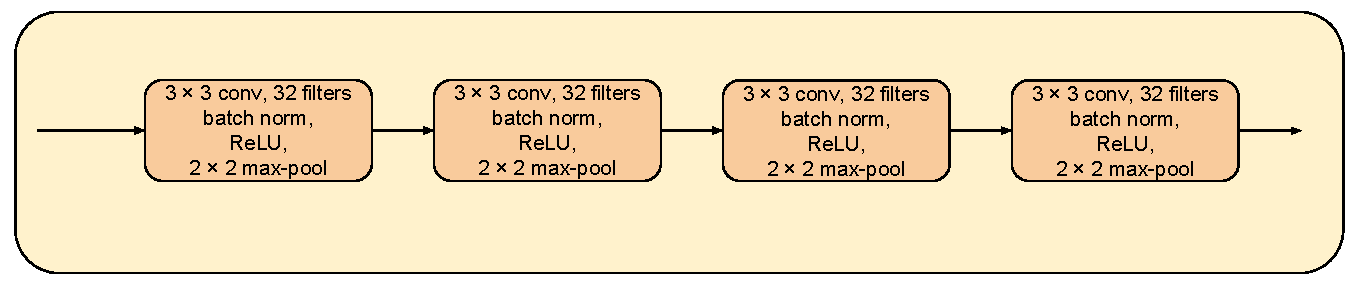
\includegraphics[width=7in]{MTL_NetArch_4CONV.pdf}
\caption{Network architecture of 4CONV}
\label{figure_netarch_4CONV}
\end{figure*}
\begin{figure*}
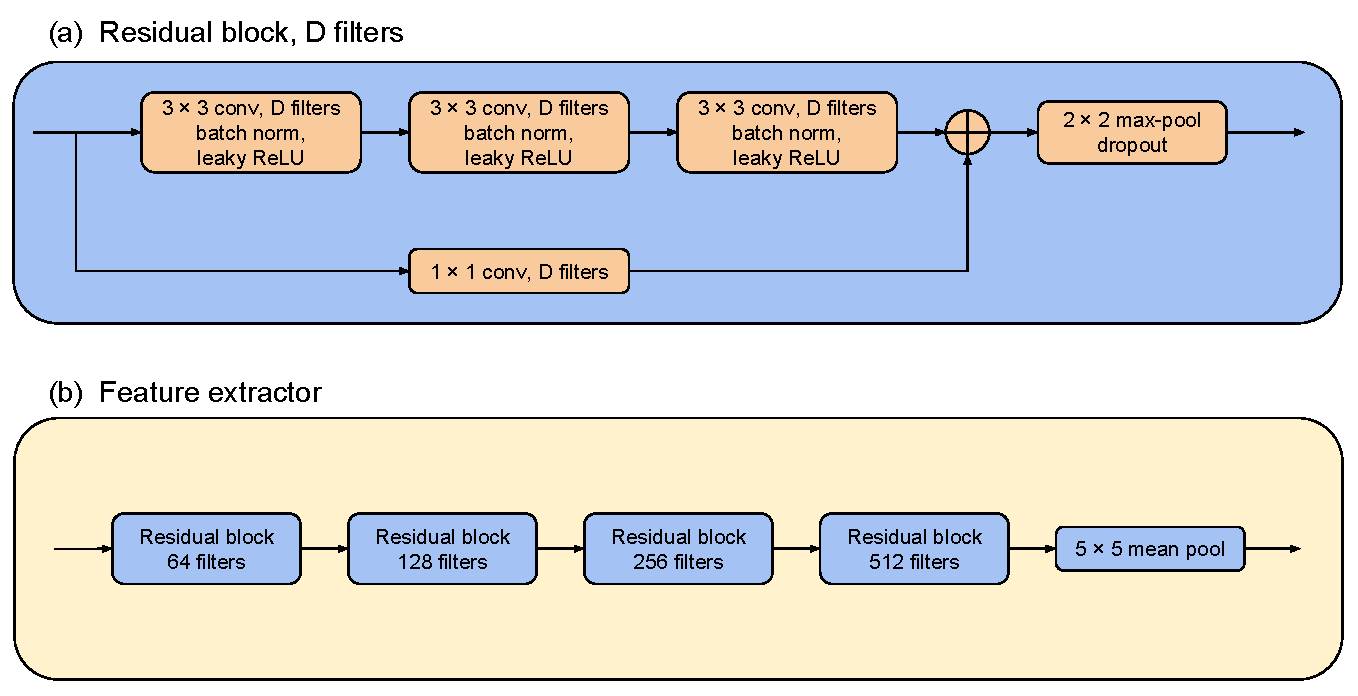
\includegraphics[width=7in]{MTL_NetArch.pdf}
\caption{Network architecture of ResNet-12}
\label{figure_netarch}
\end{figure*}



\section{Interpretation of meta-learned \emph{SS}}
\label{sec_visual}
\begin{figure*}
\centering
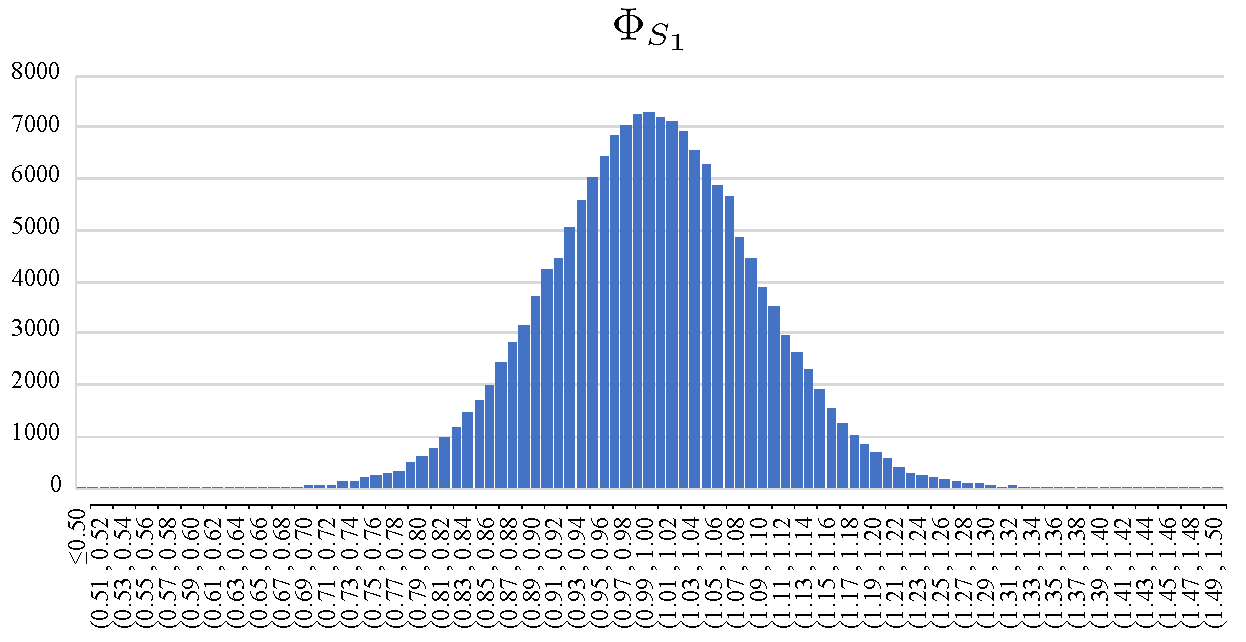
\includegraphics[height=3in]{figures/CONV_ALL.pdf}
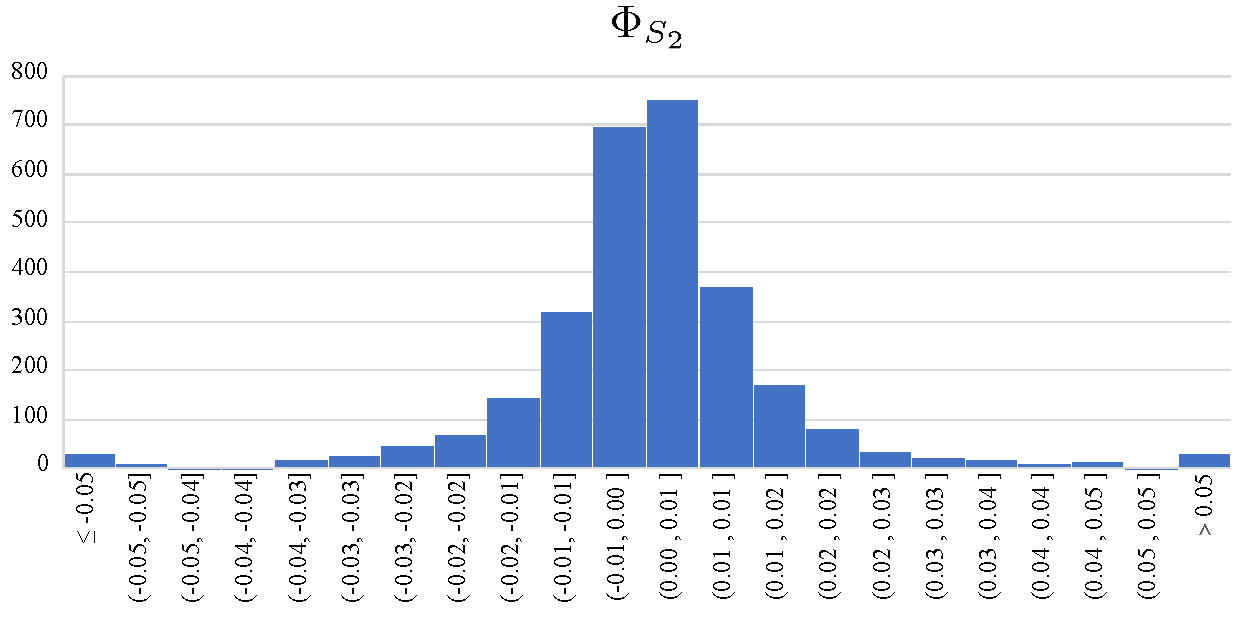
\includegraphics[height=3in]{figures/BIAS_ALL.pdf}
\caption{The statistic histograms of learned \emph{SS} parameters, taking miniImageNet 1-shot as an example setting.}
\vspace{-0.3cm}
\label{statistics}
\end{figure*}

In Figure~\ref{statistics}, we show the statistic histograms of learned \emph{SS} parameters, taking miniImageNet 1-shot as an example setting.
%
Scaling parameters $\Phi_{S_1}$ are initialized as 1 and shifting parameters $\Phi_{S_1}$ as 0. After meta-train, we observe that these statistics are close to Gaussian distributions respectively with ($0.9962$, $0.0084$) and ($0.0003$, $0.0002$) as (mean, variance) values, which shows that the uniform initialization has been changed to Gaussian distribution through few-shot learning. 
Possible interpretations are in three-fold: 1) majority patterns trained by a large number of few-shot tasks are close to the ones trained by large-scale data; 2) tail patterns with clear scale and shift values are the ones really contributing to adapting the model to few-shot tasks; 3) tail patterns are of small quantity, enabling the fast learning convergence. 


